\chapter{Resultados e Discussões}	

A caracterização do arcabouço estrutural utilizando métodos sismológicos possui problemas de unicidade de solução, como outros métodos geofísicos.  Essa falta de informação direta do objeto em estudo proporciona uma gama de soluções, entretante há inúmeros meios de se contornar essa situação. A modelagem mostra-se uma boa opção, pois consegue comprovar se a técnica utilizada tem resolução para seu objetivo.

\begin{figure}[!ht]
\centering
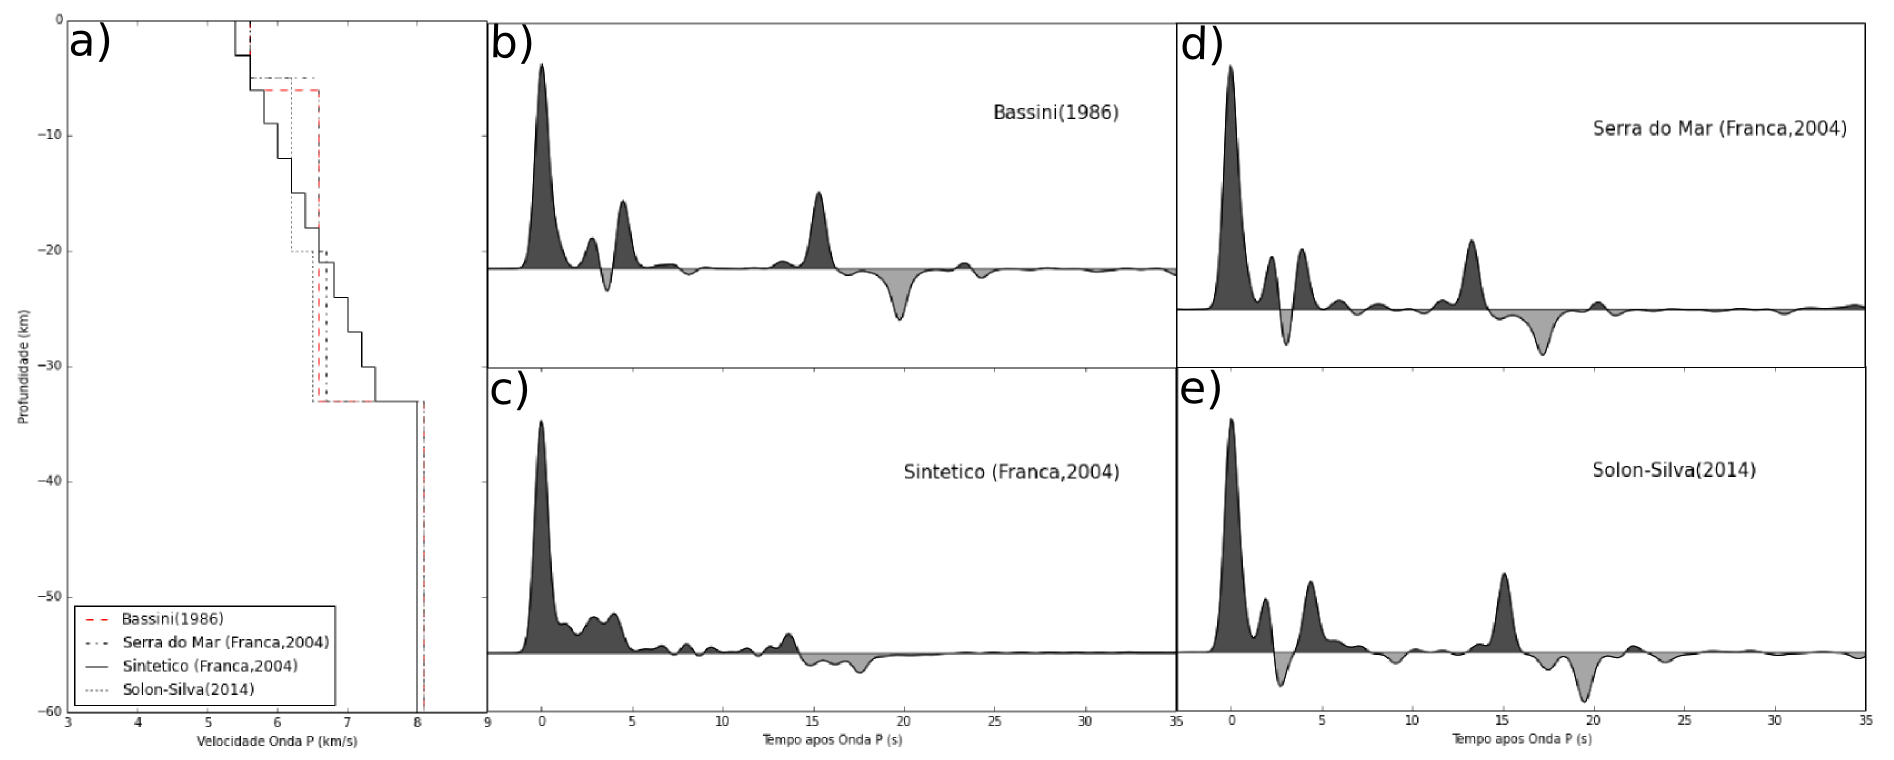
\includegraphics[scale=0.4]{modelagem_RF.png}
\caption{Funções do Receptor Sintéticas para área abrangida pelo projeto do SUBSAL segundo vários tipos de modelos de velocidade da onda P.}
\label{modelagem}
\end{figure}

Para delimitar as principais feições estruturais da área em estudo utilizou-se modelos simples, como visto na Figura \ref{modelagem}, apenas com camadas planas. Com esses modelos pretende-se mostrar que as estimativas da espessura crustal e razão $V_{p}/V_{s}$ são consistentes com os dados observados. Para a confecção e cálculo das Funções do Receptor Sintéticas aplicou-se a metodologia proposta por \cite{Ammon_waterlevel_1997}. 

Nessa medotologia os programas utilizados para criar os modelos foram "\textit{icmod}" e "\textit{vplot[s]}". A preparação dos dados foi feita pelo programa "\textit{respknt}". O programa "\textit{pwaveqn}" calculou as Funções do Receptor no domínio da frequência para os modelos pré-estabelecidos. Os parâmetros utilizados para o cálculo das Funções do Receptor estão na Figura \ref{modelagem}. Toda a demonstração da modelagem e cálculo das Funções do Receptor está disponibilizada por \cite{Ammon_waterlevel_1997} em sua página na internet.

Os modelos de velocidade da onda P ($V_{p}$) são exemplos retirados da literatura sobre a região em estudo. \cite{Bassini_1986} foi o primeiro a estimar a estrutura crustual para a região da Faixa Riberia, então neste trabalho utilizou-se o modelo de velocidade sísmica para a região da Serra do Mar, como observado na Figura \ref{modelagem}. Mais tarde, \cite{sand_franca_crustal_2004} re-compilou os dados de \cite{Bassini_1986} e propôs um novo modelo de velocidade sísmica da região da Serra do Mar, como visto na Figura \ref{modelagem}. Recentemente \cite{flora_solon_ancient_2013} e \cite{Silva_2014} geraram resultados da estrutura crustal da região em estudo através dos métodos magnetométrico e gravimétrico, respectivamente. Baseando-se nesses resultados, organizou-se um modelo de velocidade sísmica para a região em estudo, como visto na Figura \ref{modelagem}. Uma opção de modelo sísmico levantada por \cite{sand_franca_crustal_2004} é o modelo Sintético, mostrado na Figura \ref{modelagem}. Neste modelo o autor considera que a variação das propriedades físicas da região aumenta progressivamente com a profundidade.

\begin{figure}[!ht]
\centering
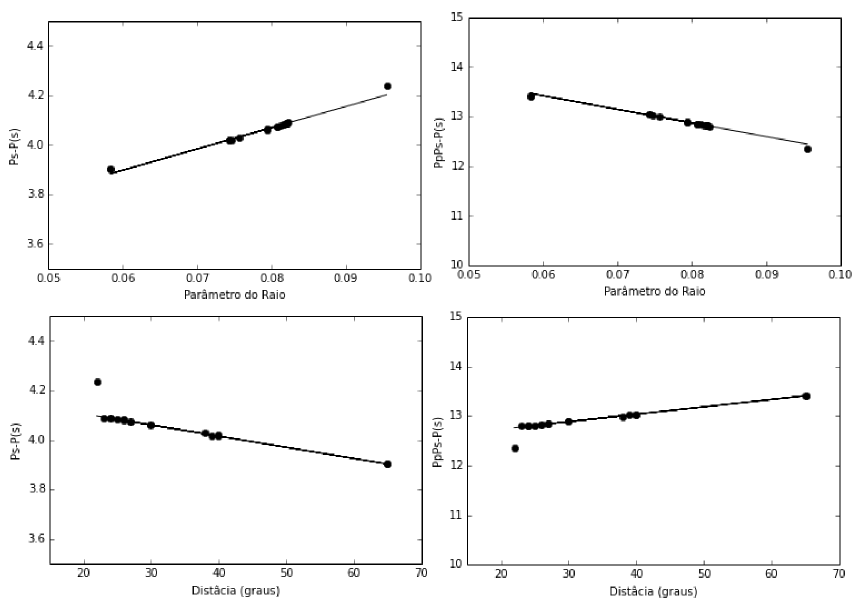
\includegraphics[scale=0.7]{tempo_teorico_modelo_tauptime.png}
\caption{Tempos teóricos para a reflexão $Ps$ (gráficos à esquerda) e fases $PpPs$ segundo o modelo de \cite{kennet_iaspei_1991}. Os tempos estão classificados segundo o parâmetro do raio e as distâncias epicentrais.}
\label{tauptime}
\end{figure}


A Figura \ref{RF_SLP01} mostra as Funções do Receptor obtidas de vários eventos na estação SLP01. Estes sinais estão normalizados pela amplitude do primeiro pico. O primeiro pick é a chegada da onda P direta, já o segundos, por volta de 5 segundos, e a onda P convertida em onda S na discontinuidade de Moho. As multiplas $PpPs$ e $PpSs+PsPs$ tem uma amplitude menor que a onda P convertida em S($Ps$). 

\begin{figure}[!ht]
\centering
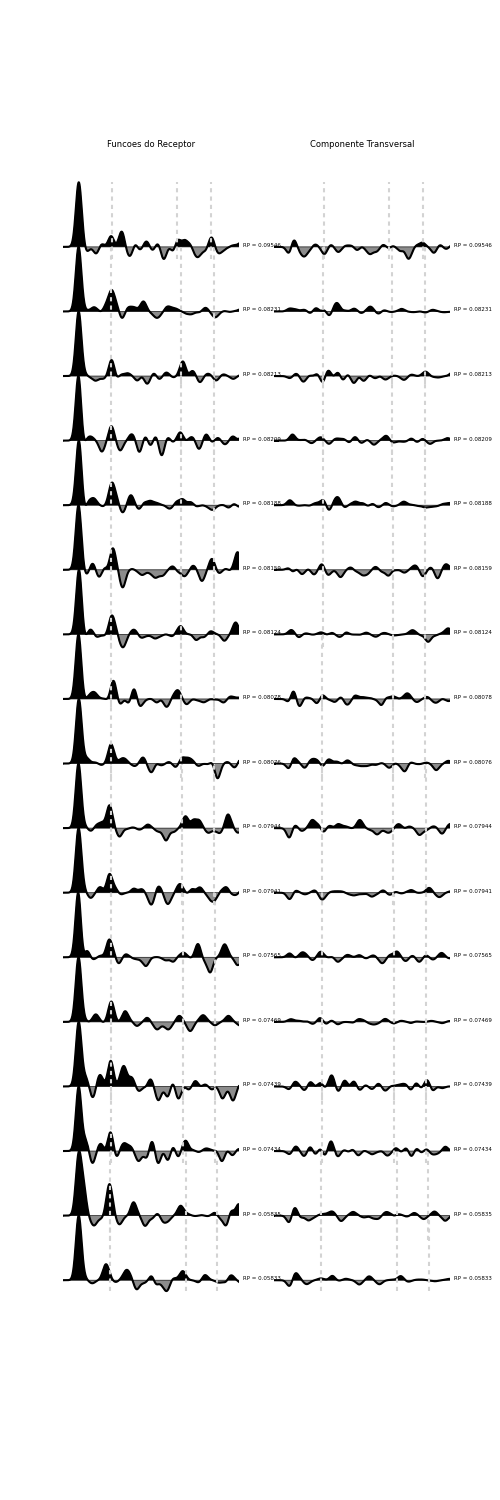
\includegraphics[scale=0.35]{RF_SLP01.png}
\caption{}
\label{RF_SLP01}
\end{figure}

%________________AJUSTAR________________________________


Nota-se na Figura \ref{RF_SLP01} que a discontinuidade de Moho estimada é maior no interior do continente do que na região costeira, corroborando com os dados de \cite{Assumpcao_America_2013}, \citep{Assumpcao_Brazil_2013} e \cite{van_der_meijde_gravity_2013} . Identfica-se sinais precursores a Moho, por volta de 2 a 4 segundos, que variam ao longo do perfil. Estes sinais podem ser relacionados com uma interface com um alto contraste de propriedade fisica. O pulso negativo antes de 5 segundos indica, segundo as modelagens propostas na Figura \ref{modelagem}, uma camada com baixa velocidade.



The uncertainties of data are linked to the quality and the quantity of the Receiver Functions. The estimated values of the Moho depth for each station were linearly interpolated to generate a regional map, shown in Figure. In order to improve the interpolation, we added data from \citep{assumpcao_crustal_2013}. In Figure \ref{figura7}, we can see the Moho thinning in direction to the east.

The Figure \ref{figura5} shows a section of Receiver Functions obtained from several events and normalized by the amplitude of the first peak. The first peak is the direct P-wave arrival, the second highest, around 5 seconds, is the P wave converted to S wave in the Moho discontinuity. 


\begin{figure}[!ht]
\centering
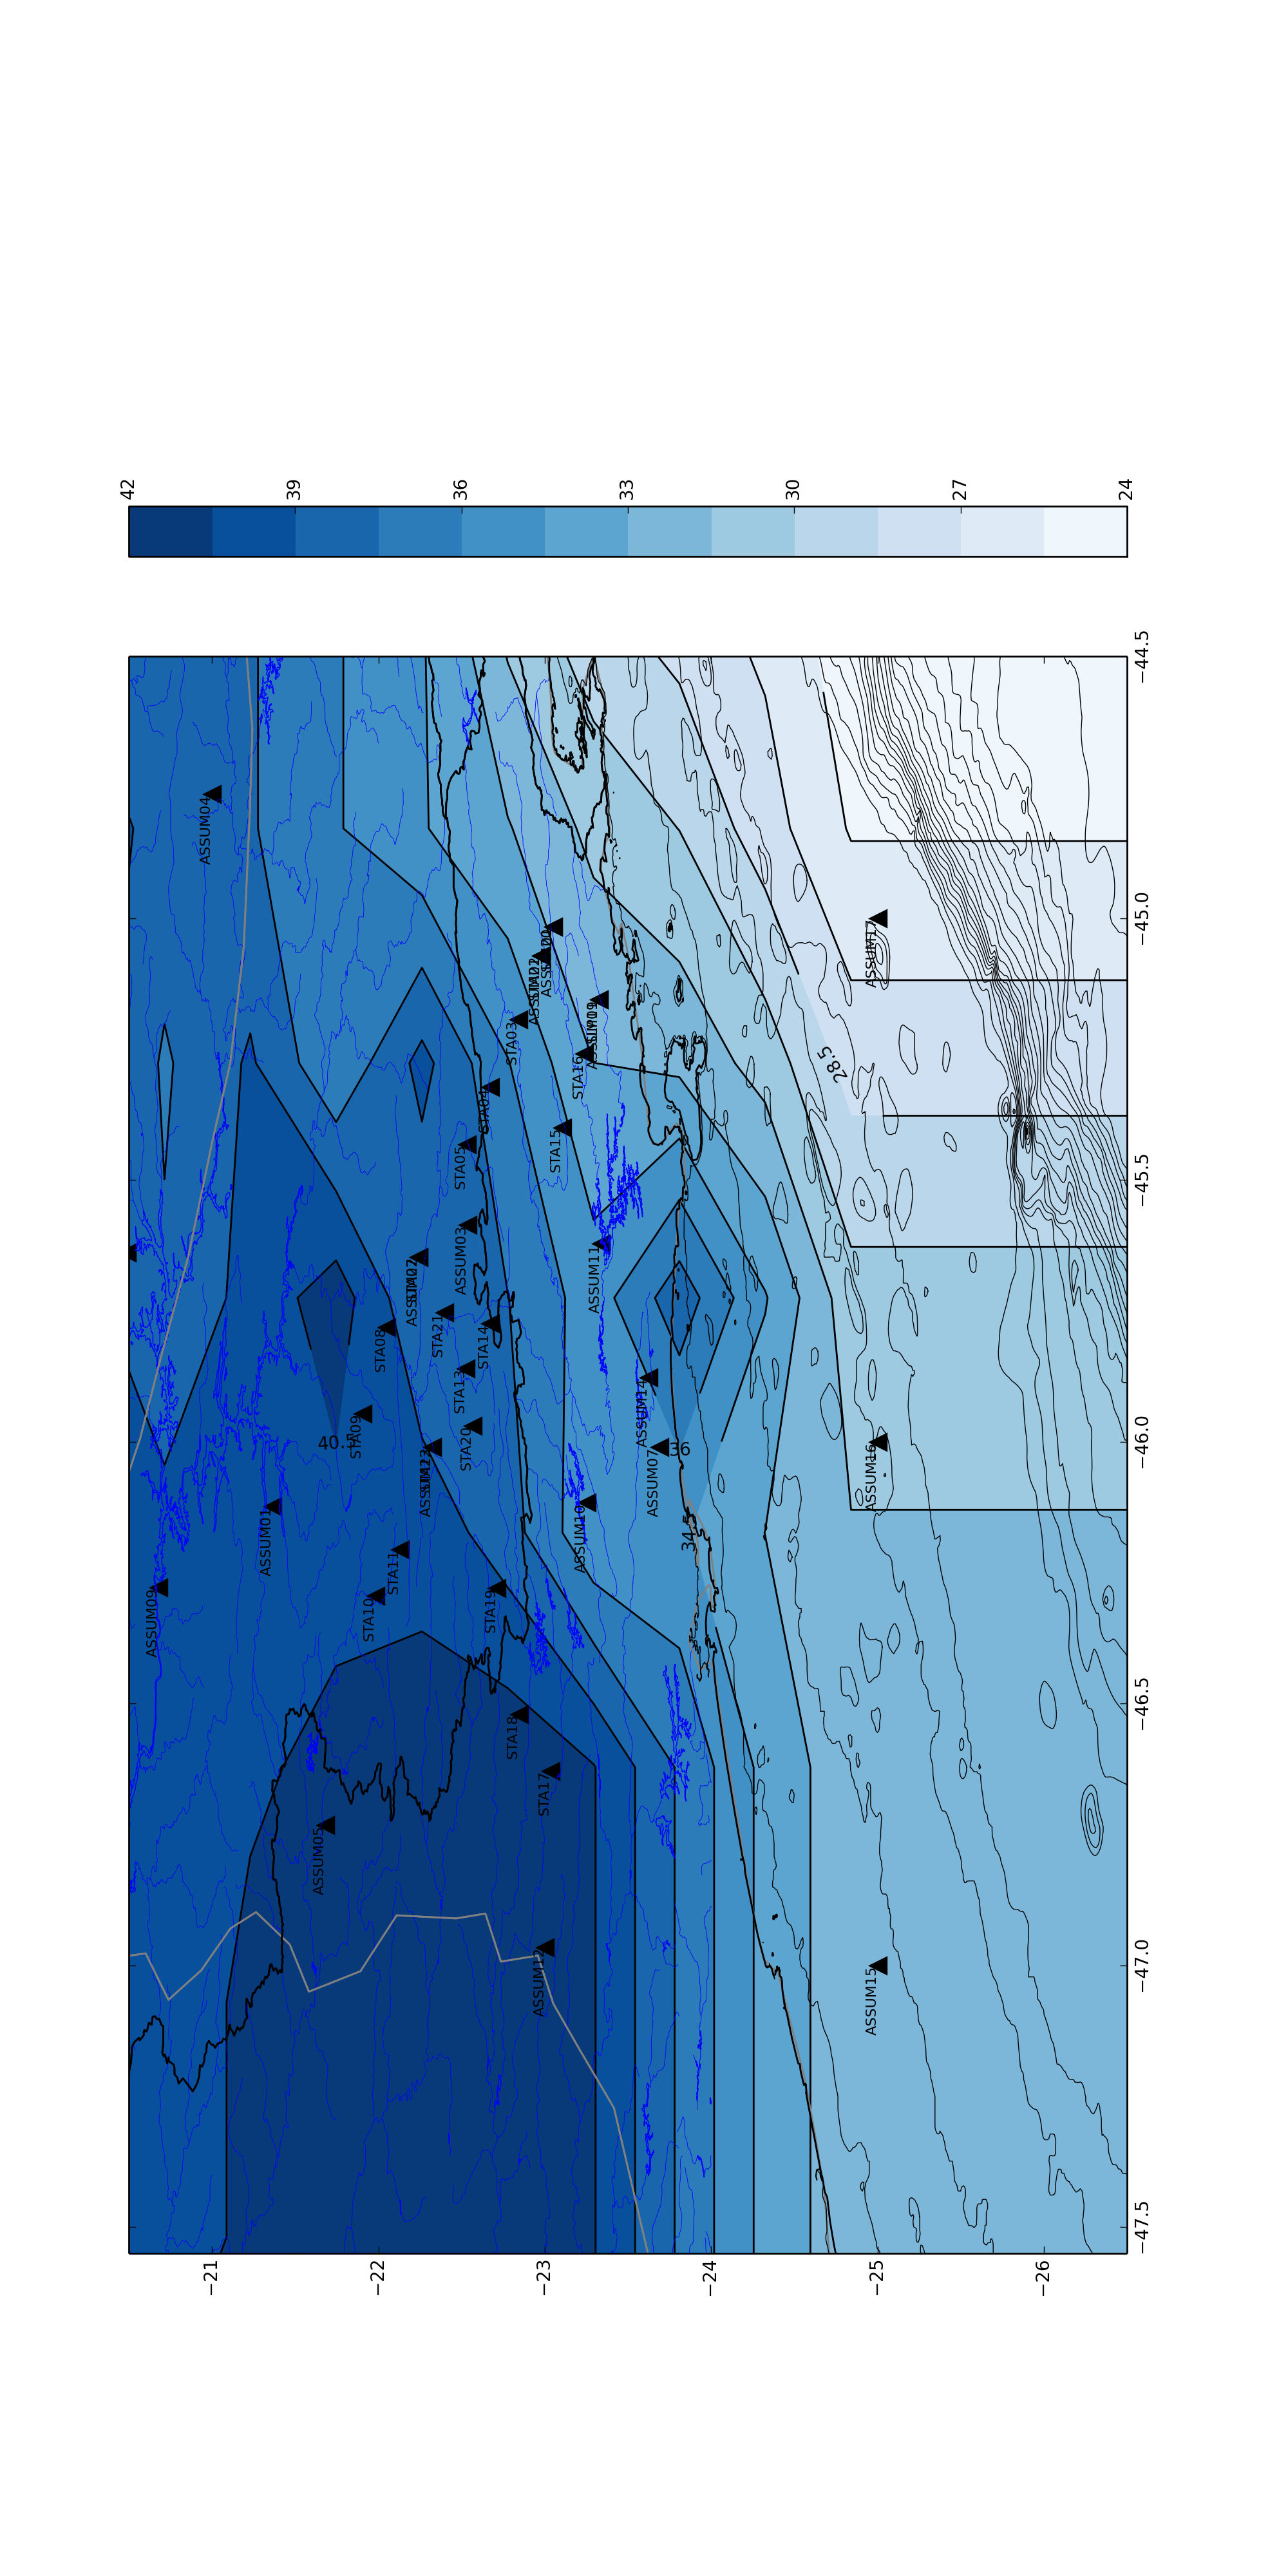
\includegraphics[scale=0.2]{Interpolacao_Linear.png}
\caption{}
\label{RF_perfil_NW}
\end{figure}

The uncertainty, shown in Table \ref{tabela} are linked to quality and quantity of the Receiver Functions. A important phase is the selection of the best Receiver Functions, because the data quality is preponderant over the quantity. The uncertainty associated a each one of obtained parameters by the method Hk and estimated generally by "bootstrap" method, developed for  \citep{efron_statistical_1991}. From the original set of Receiver Functions the program generates subsets containing traces randomly selected. These method is repeated for each subsets, resulting in a parameter set H and $v_{p}/v_{s}$ .Mean and standard deviation from the values provide us a mean value and an estimate of the uncertainty associated to determination. There is no rule for determining the number subsets that must be generated, the crucial is search a value that makes the estimative stabilize,  including uncertainties. In general we use a value between 100 and 200 subsets depending on the amount de traces available during the “bootstrap”.

The calculated values of the Moho depth for each station were linearly interpolated to generate a regional map, shown in the Figure \ref{figura7}. To improve the interpolation, we added data from \citep{assumpcao_crustal_2013}. In the Figure \ref{figura7} we can see the Moho thinning in direction to east, reinforcing the proximity with the oceanic crust.

\begin{figure}[!ht]
\centering
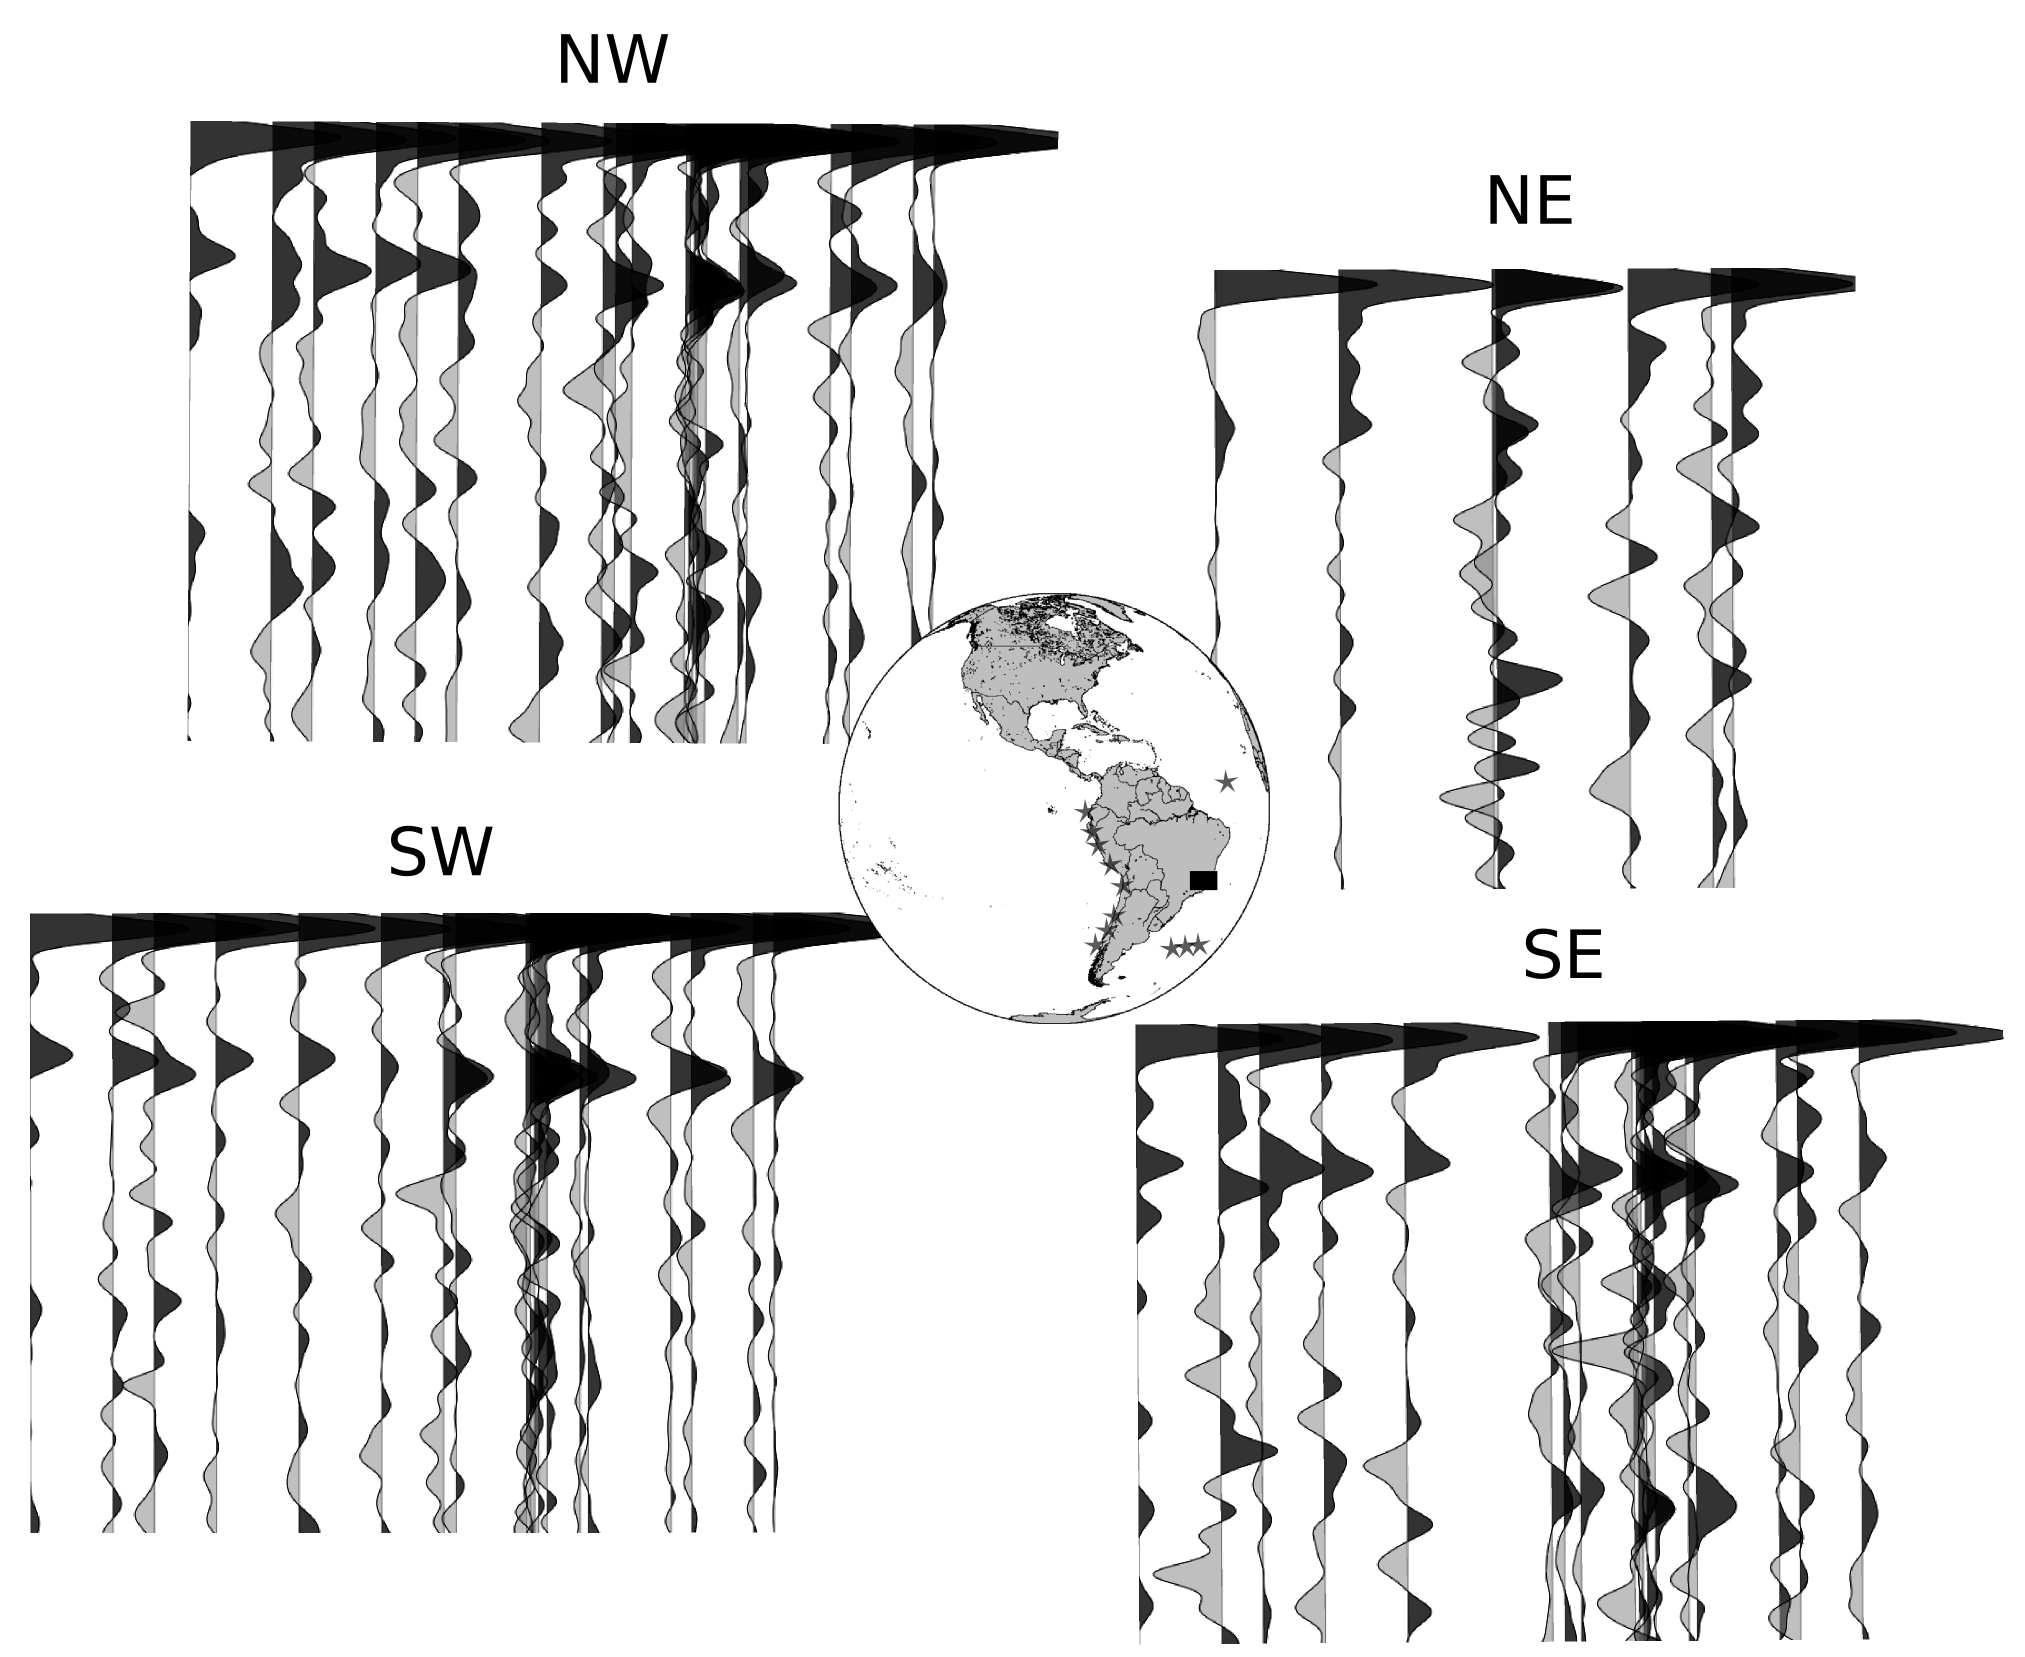
\includegraphics[scale=0.5]{RF_azimute.png}
\caption{}
\label{RF_perfil_NW}
\end{figure}

